\section{Aquiring a New 3D Printer}
The Department of Engineering Cybernetics is renting office space at Nyhavna to accommodate the growing number of employees.
Due to this relocation, I have to travel to Gløshaugen, which is a 40-minute walk away, if I want to use the workshops there.
During the pre-project most of the parts were with the laser cutter at \gls{ov}, as is could be done in a single session.
The process of using a 3D printer was more inconvenient as it necessitated two separate trips for each print job: one to initiate the print and another to stop it.
If the print failed, the process had to be repeated.
Based on this experience, it was deemed necessary to have a 3D printer available at Nyhavna.
Argumentation was put forward to the department, and I got funding to acquire a 3D printer at Nyhavna.

\subsection{Choice of printer}
Selecting a 3D printer is a difficult task as there are many different options available.
The main requirements for the printer were:
\begin{enumerate}
    \item \textbf{Availability:} The printer should be available for purchase.
    \item \textbf{Price:} The printer should be within the assigned budget.
    \item \textbf{Reliability:} The printer should be reliable and require little maintenance.
    \item \textbf{Print quality:} The printer should be able to print high-quality parts.
    \item \textbf{Print volume:} The print volume should be able to print relatively large parts.
    \item \textbf{Multi filament printing:} The printer should ideally be able to print with multiple filaments simultaneously.
\end{enumerate}

After some research, contenders were the Bambu Lab X1 and the Snapmaker J1, but as the X1 was not available for purchase at the time, the Snapmaker J1 was selected.
The J1 is an IDEX printer, meaning it has two independent extruders that can print simultaneously or be used to print with two different materials without changing the filament between each layer.

\subsection{Choice of Materials}
PETG was chosen as the primary printing material due to its ease of use, along with its durability and resistance to high temperatures, UV light, and water \cite{oconnellPETGVsPLA2023}.
For the supports, PLA was selected as the material of choice.
Printing supports in a different material offer advantages such as easier removal and smoother surfaces at the intersection points, as the bonding between different plastics is weaker.
Although special breakaway filament was considered, PLA was ultimately chosen due to its cost-effectiveness, widespread availability, and successful use by others in similar applications \cite{SupportFilamentPETG2023}.

\subsection{Printing Workflow}
Figure \ref{fig:3dp_workflow} shows the full workflow for 3D printing parts.
First, parts are designed in \gls{fusion}, a \gls{cad} software developed by Autodesk.
The design process is documented in Chapter 2 of the \preproject.
After a part is designed it is sent to Cura slicer.
A slicer is a program that translates the 3D model into a set of instructions for the printer, called \gls{gcode}.
This \gls{gcode} is saved and opened in a program called \gls{luban} which can send it to the printer over the network.
It was not possible to do this over Eduroam, and the printer does not have an ethernet port, so a local network was set up using a separate router.
The printer progress is monitored in \gls{luban} over the network.
Using \gls{luban}, directly to slice the model was possible, but it lacked some of the advanced features of Cura, most notably related to the support tree structure.


\begin{figure}[H]
    \centering
    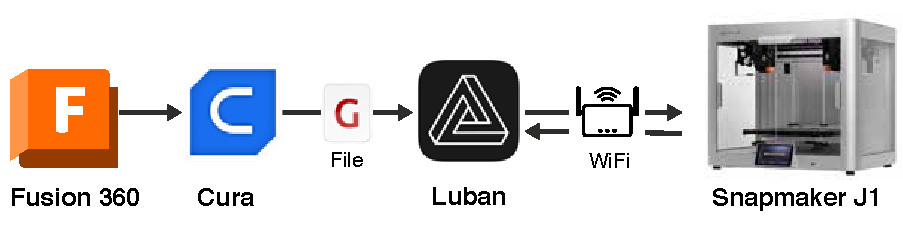
\includegraphics[width=\textwidth]{figures/3d_print/pipeline.pdf}
    \caption{3D-printing workflow \cite{autodeskFusion360Logo} \cite{delaragoCuraLogo2022} \cite{jupi007GcodeIconProposal2020} \cite{snapmakerSnapmakerLogo2020} \cite{snapmakerSnapmakerJ1High}}
    \label{fig:3dp_workflow}
\end{figure}

\subsection{Calibrating the Printer}

A significant amount of time was dedicated to calibrating the printer and fine-tuning the slicer settings to achieve the best possible print quality.
The calibration process involved creating multiple small test prints, identifying areas for improvement, such as stringing or uneven surfaces, and seeking solutions from various online resources.
As a newcomer to 3D printing, I found the tutorials available on All3DP to be particularly valuable in understanding how to address various issues \cite{all3dpBasicsArchives}.
In addition, the \textit{AutoTowers Generator} extension in Cura played a significant role in tuning the parameters such as temperature, flow rate, and fan speed, as it allowed for testing a linear range of values in a single print as shown in Figure \ref{fig:auto_towers} \cite{kartchnerAutoTowersGeneratorUltimaker2022}.
The complete set of parameters that were adjusted during the calibration process can be found in Section \ref{sec:cura_configurations} in the appendix.

During the calibration process, two specific issues were encountered that are worth highlighting.

\begin{figure}[H]
    \centering
    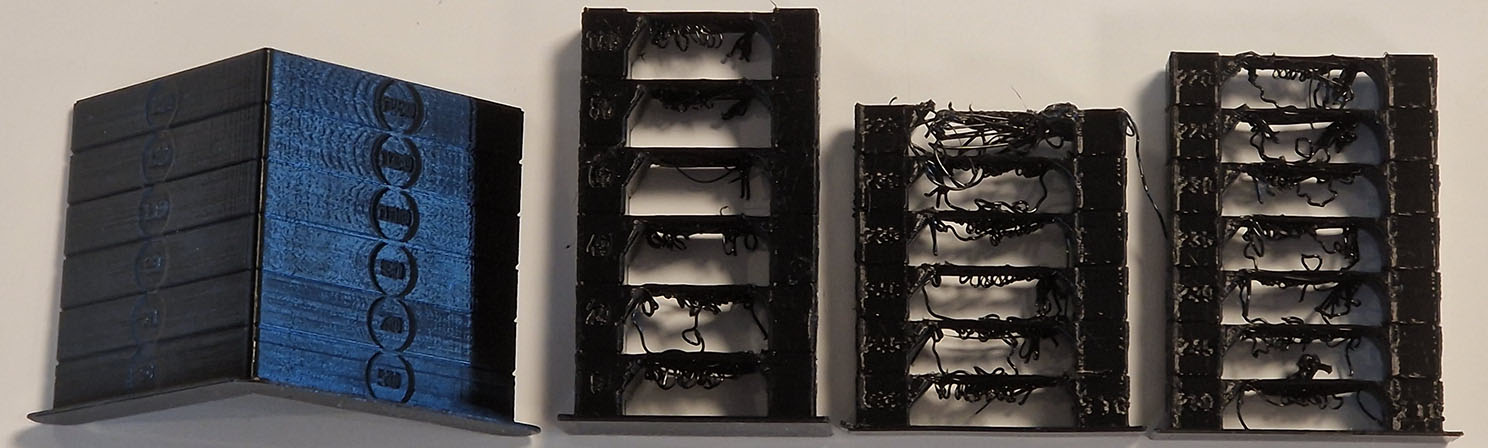
\includegraphics[width=\textwidth]{figures/3d_print/auto_towers.jpg}
    \caption{Some auto towers generated during the calibration process.
        The left sample shows how the speed affects the surface quality, while the others show early attempts at tuning fan speed and temperature.}
    \label{fig:auto_towers}
\end{figure}


\subsubsection{M109 - Wait for Hotend Temperature}
When both extruders are used during printing, a siginificant dealy occurs at every switch.
It was discovered that it was caused by the \code{M109} commends in the generated \gls{gcode}, which tells the printer to wait for the hot end to reach target temperature \cite{thinkyheadWaitHotendTemperature2023}.
By default the extruders are set to cool down to their stand-by temperature when not in use and heat up again when its their turn to print.
As the extruders started heating up to late, a significant waiting time would occur.
Following a tip from a threadpost, the \code{Printer Settings} plugins was used in curea to decrease the \code{Heat Up Speed} and \code{Cool Down Speed} values used to calculate when the heating should start \cite{valiantReplyStandbyTemperature2022} \cite{fieldofviewPrinterSettingsUltimaker}.
This reduced the waiting time but did not remove it entierly, as the printer would wait for some time even if the set temperature was already reached.
The final solution was then to simply set the stand by temperatures equal to the printing temperatures witch resulted in GCode without \code{M109} commands between each extruder change.


\subsubsection{Initial Layer Flow}
One issue was that material had a tendency to build up around the nozzle during the first layer as visualized in Figure \ref{fig:first_layer_buildup}.
This sometimes resulted in a dirty nozzle and sometimes the nozzle would pull the material with it, resulting in a failed print.
Other people on the Snammaker forum have also reported this issue, without finding a clear solution \cite{artezioFinerAdjustmentsOffset2021} \cite{napsZHeightCalibrationOffset2023}.

After attempting the printer calibration process multiple times without resolving the issue, the next approach was to manually adjust the z-offset.
Unfortunately, the settings tab of the \gls{j1} did not provide any parameter for adjusting the z-offset.
The issue then solved by increasing the initial layer height in the slice profile and and reducing the initial layer flow until the issue disappeared, which happened at a flow rate of $75\%$.
Subsequently, it was revealed that the z-offset adjustment on the \gls{j1} is indeed possible, albeit only accessible during the printing process, for unknown reasons.
It was confirmed that the modifications made to the z-offset persisted between prints.

\begin{figure}[H]
    \centering
    
\includegraphics[width=\textwidth]{figures/3d_print/first_layer_buildup.pdf}
    \caption{Illustration of material buildup on the first layer.}
    \label{fig:first_layer_buildup}
\end{figure}